\usepackage{color}
\definecolor{lightgray}{rgb}{0.98, 0.98, 0.98}
\definecolor{darkgray}{rgb}{0.4, 0.4, 0.4}
%\definecolor{purple}{rgb}{0.65, 0.12, 0.82}
\definecolor{editorGray}{rgb}{0.95, 0.95, 0.95}
\definecolor{editorOcher}{rgb}{1, 0.5, 0} % #FF7F00 -> rgb(239, 169, 0)
\definecolor{editorGreen}{rgb}{0, 0.5, 0} % #007C00 -> rgb(0, 124, 0)
\definecolor{orange}{rgb}{1,0.45,0.13}		
\definecolor{olive}{rgb}{0.17,0.59,0.20}
\definecolor{brown}{rgb}{0.69,0.31,0.31}
\definecolor{purple}{rgb}{0.38,0.18,0.81}
\definecolor{lightblue}{rgb}{0.1,0.57,0.7}
\definecolor{lightred}{rgb}{1,0.4,0.5}
\usepackage{upquote}
\usepackage{listings}



% CSS
\lstdefinelanguage{CSS}{
  keywords={display,
  text-decoration,font-family,
  background-color,box-shadow,color,background-image:,margin,padding,font,weight,display,position,top,left,right,bottom,list,style,border,size,white,space,min,width,
  transition:, transform:, transition-property, transition-duration, transition-timing-function}, sensitive=true, morecomment=[l]{//}, morecomment=[s]{/*}{*/},
  morestring=[b]',
  morestring=[b]",
  alsoletter={:},
  alsodigit={-}
}

% JavaScript
\lstdefinelanguage{JavaScript}{
  morekeywords={typeof, new, true, false, catch, function, return, null, catch, switch, var, if, in, while, do, else, case, break},
  morecomment=[s]{/*}{*/},
  morecomment=[l]//,
  morestring=[b]",
  morestring=[b]'
}

\lstdefinelanguage{HTML5}{
  language=html,
  sensitive=true,	
  alsoletter={<>=-},	
  morecomment=[s]{<!-}{-->},
  tag=[s],
  otherkeywords={
  % General
  >,
  % Standard tags
	<!DOCTYPE,
  </html, <html, <head, <title, </title, <style, </style, <link, </head, <meta, />,
	% body
	</body, <body,
	% Divs
	</div, <div, </div>, 
	% Paragraphs
	</p, <p, </p>,
	% scripts
	</script, <script,
  % More tags...
  <canvas, /canvas>, <svg, <rect, <animateTransform, </rect>, </svg>, <video, <source, <iframe, </iframe>, </video>, <image, </image>, <header, </header, <article, </article
  },
  ndkeywords={
  % General
  =,
  % HTML attributes
  charset=, src=, id=, width=, height=, style=, type=, rel=, href=,
  % SVG attributes
  fill=, attributeName=, begin=, dur=, from=, to=, poster=, controls=, x=, y=, repeatCount=, xlink:href=,
  % properties
  margin:, padding:, background-color:, text-decoration:, color:, display:,
  box-shadow:, font-family:, width:, height:, background-image:, border:, top:,
  left:, position:, width:, height:, margin-top:, margin-bottom:, font-size:, line-height:,
	% CSS3 properties
  transform:, -moz-transform:, -webkit-transform:,
  animation:, -webkit-animation:,
  transition:,  transition-duration:, transition-property:, transition-timing-function:,
  }
}

\lstdefinestyle{htmlcssjs} {%
  % General design
%  backgroundcolor=\color{editorGray},
  basicstyle={\footnotesize\ttfamily},   
  frame=b,
  % line-numbers
  xleftmargin={0.75cm},
  numbers=left,
  stepnumber=1,
  firstnumber=1,
  numberfirstline=true,	
  % Code design
  identifierstyle=\color{black},
  keywordstyle=\color{blue}\bfseries,
  ndkeywordstyle=\color{editorGreen}\bfseries,
  stringstyle=\color{editorOcher}\ttfamily,
  commentstyle=\color{brown}\ttfamily,
  % Code
  language=HTML5,
  alsolanguage=JavaScript,
  alsodigit={.:;},	
  tabsize=2,
  showtabs=false,
  showspaces=false,
  showstringspaces=false,
  extendedchars=true,
  breaklines=true,
  % German umlauts
  literate=%
  {Ö}{{\"O}}1
  {Ä}{{\"A}}1
  {Ü}{{\"U}}1
  {ß}{{\ss}}1
  {ü}{{\"u}}1
  {ä}{{\"a}}1
  {ö}{{\"o}}1
}
%
\lstdefinestyle{py} {%
language=python,
literate=%
*{0}{{{\color{lightred}0}}}1
{1}{{{\color{lightred}1}}}1
{2}{{{\color{lightred}2}}}1
{3}{{{\color{lightred}3}}}1
{4}{{{\color{lightred}4}}}1
{5}{{{\color{lightred}5}}}1
{6}{{{\color{lightred}6}}}1
{7}{{{\color{lightred}7}}}1
{8}{{{\color{lightred}8}}}1
{9}{{{\color{lightred}9}}}1,
basicstyle=\footnotesize\ttfamily, % Standardschrift
numbers=left,               % Ort der Zeilennummern
%numberstyle=\tiny,          % Stil der Zeilennummern
%stepnumber=2,               % Abstand zwischen den Zeilennummern
numbersep=5pt,              % Abstand der Nummern zum Text
tabsize=4,                  % Groesse von Tabs
extendedchars=true,         %
breaklines=true,            % Zeilen werden Umgebrochen
keywordstyle=\color{blue}\bfseries,
frame=b,
commentstyle=\color{brown}\itshape,
stringstyle=\color{editorOcher}\ttfamily, % Farbe der String
showspaces=false,           % Leerzeichen anzeigen ?
showtabs=false,             % Tabs anzeigen ?
xleftmargin=17pt,
framexleftmargin=17pt,
framexrightmargin=5pt,
framexbottommargin=4pt,
%backgroundcolor=\color{lightgray},
showstringspaces=false,      % Leerzeichen in Strings anzeigen ?
}%
%

% !TEX root = ../Projektdokumentation.tex
\section{Implementierungsphase} 
\label{sec:Implementierungsphase}
Die Implementierung der Website geschieht in 3 Schritten: 
Die Entwicklung eines HTML Dummies unter Verwendung von \acs{HTML}5 und
\ac{CSS}3 \bzw  Less nach \acs{BEM} Methodik. Folgend die Ausarbeitung
der JavaScript \bzw jQuery Funktionalität im Frontend. Anschließend die Integration in 
das firmeneigene Content Management System \ct, sowie dessen Anpassung.

\subsection{Implementierung des HTML Dummys}
\label{sec:ImplementierungDummy}

Das die vertikale Darstellung der Elemente auf der Seite meistens mit der
Position im \ac{DOM} korrespondiert, wurde bei der Entwicklung des HTML Dummys
die Vorgehensweise Top-Bottom gewählt. Bei der Auswahl der \ac{HTML} Elemente
für die Container werden die semantischen \ac{HTML}5 Tags <article>, <section>,
<nav>, <aside>, \usw priorisiert. Der Einsatz von semantischen Tags steigert
die Suchmaschinenoptimierung und verbessert die \ac{DOM} Übersicht für den
Entwickler. \ac{W3C} schreibt vor, generische Container die nur für das Styling
gebraucht werden in Form von <div> Tags zu verwenden. Semantische Elemente sind
für relevante und bedeutsame Elemente aufzubewahren.


Das Top-Bottom Verfahren beruht sich auf die schrittweise Umsetzung der
\ac{HTML}-Seite in seperaten Blöcken. Aufgrund des angewandten Desktop
First Konzeptes, welches die Entstehung der Desktop Version als erstes vorsieht,
werden die Blöcke im nachhinein für die mobile Version mithilfe von Media
Queries optimiert. Zu beachten sind die in diesem Projekt benötigten Breakpoints für die
Desktopansicht, Tabletansicht und Smartphoneansicht. Unter Breakpoints versteht
man die Breite des Browserfensters in Pixel, von der die Position einzelner
Elemente abhängig sind. Die Pixelwerte dazu wurden unverändert von Bootstrap
übernommen. Eine grobe Strukur des \ac{DOM} ist im \Anhang{listing:DOM} zu
finden. 

\subsubsection{Umsetzung der BEM Methodik anhand eines Beispieles}
\label{sec:BEMExample}
Um den Code leserlicher und skalierbarer zu machen,
werden die Klassen in \acs{BEM} nach einem bestimmten Muster benannt. 
Die Konvention dazu ist \lstinline{.Block__Element--Modifier}. 
Bei der Umsetzung von \ac{BEM} ist ein umfangreiches Studieren der Screendesigns
unumgänglich. Dabei versucht man verschiedene Gestaltungselemente die sich
ähnlich sind (Varianten) zu einer Komponente zusammen zu fassen. 
Die Standardvariante ist meistens die, die am häufigsten vor kommt oder am
geringsten stilisiert wurde. 

Das in sich geschlossene Gestaltungselement wird als Block bezeichnet. 


\begin{figure}[ht]
\caption{Block}
\center{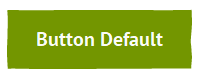
\includegraphics[scale=0.9]{Bilder/button-default.png}}
\end{figure}
\\
\begin{lstlisting}[style=htmlcssjs, backgroundcolor = \color{lightgray},
caption=BEM -- Block Default (HTML)] 
<a href="#" class="button">Button Default</a>
\end{lstlisting}

\begin{lstlisting}[style=htmlcssjs, backgroundcolor = \color{lightgray},
caption=BEM -- Block Default (CSS)]
.button {
  height: initial;
  position: relative;
  display: inline-block;
  padding: 15px 30px;
  font-size: 20px;
  color: @color-white;
  text-decoration: none;
  background-image: url('../img/svg/button.svg');
  [...]
}
\end{lstlisting}
\clearpage
Zur Veränderung der Optik werden Blöcke sowie Elemente mit Modifier ergänzt
(=Varianten).

\begin{figure}[ht]
\caption{Block mit Modifier}
\center{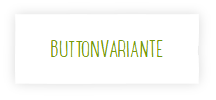
\includegraphics[scale=0.9]{Bilder/button-mod.png}}
\end{figure}

\begin{lstlisting}[style=htmlcssjs, backgroundcolor = \color{lightgray},
caption=BEM -- Block mit Modifier (HTML)]
<a href="#" class="button button--white">Buttonvariante</a>
\end{lstlisting}

\begin{lstlisting}[style=htmlcssjs, backgroundcolor = \color{lightgray},
caption=BEM -- Modifier (CSS)] 
.button--white {
  background-color: white;
  padding: 37px 50px 31px 50px;
  font-family: @font-LunchBox-Light;
  color: @color-primary;
  box-shadow: 0px 0px 10px 0px rgba(0,0,0,0.2);
}

\end{lstlisting}

Die Elemente innerhalb eines Blockes werden simpel als Elemente bezeichnet.

\begin{figure}[ht]
\caption{Block mit Element}
\center{
\includegraphics[scale=0.9]{Bilder/button-elem.png}}
\end{figure}

\begin{lstlisting}[style=htmlcssjs, backgroundcolor = \color{lightgray},
caption=BEM -- Block mit Element (HTML)]
<a href="#" class="button button--white">
	<i class="button__icon button__icon--facebook"></i>
	Gefällt mir
</a>
\end{lstlisting}

\begin{lstlisting}[style=htmlcssjs, backgroundcolor = \color{lightgray},
caption=BEM -- Element (CSS)]
.button__icon {
  background-image: url('../img/svg/fb-icon.svg');
  width:24px;
  height:24px;
}
\end{lstlisting}


\subsection{Implementierung der Javascript Funktionalitäten}
\label{sec:ImplementierungJS}
Durch das Scrollen nach unten verkleinert sich das Logo soweit, so dass das
Logo  den weißen Bereich (Navbar) nicht überschreitet. Dies wird mit dem
Hinzufügen einer Element-Modifier Klasse \\
(\lstinline{.navbar__brand--minimized}) bewerkstelligt.
\\
\begin{lstlisting}[style=htmlcssjs, backgroundcolor = \color{lightgray},
caption=Logominimierung beim Scrollen]
    $(document).scroll(function () {
        if ($(document).scrollTop() > 0) {
            $('.navbar__brand').addClass('navbar__brand--minimized');
        } else {
            $('.navbar__brand').removeClass('navbar__brand--minimized');
        }
     }).trigger("scroll");     
\end{lstlisting}

Ein Eventhandler wird an das Scroll-Event des Window-Objekts gebunden.
Wenn die Scrollposition größer gleich der oberen Kante des Browserfensters ist
(>0px), wird dem Logo die Klasse \lstinline{.navbar__brand--minimized}
hinzugefügt. Ansonsten wird diese Klasse im Else-Zweig entfernt.
Die Klasse selber beinhaltet Styles zur animierten Skalierung des Logos.

Bei der Navigation wurde aufgrund seiner hohen Komplexität, auf die schon
fertige Dropdownfunktion des Frameworks Bootsrap verzichtet. Ein weiteres
Problem ist, dass die Bootstrap Funktionalität keine Möglichkeit eines
Subdropdowns unterstützt. Das Skript dazu ist im \Anhang{app:Dropdown} zu
finden.

\subsection{Implementierung des Content Management System}
\label{sec:ImplementierungCMS}

Nach der vollständigen Umsetzung des \ac{HTML} Dummys mit rein statischen
Testinhalt beginnt die Integration des \ac{CMS}. Die \mh setzt auf die
firmeninterne Lösung conTRANCE v6. Der erste Schritt ist der Pull \bzw Export
des letzten conTRANCE Releases aus GIT. Die Dateien des HTML Dummys werden
in die conTRANCE Dateienstruktur aufgenommen. Die Datenbanktabellen des
\ac{CMS} werden vom Enticklungsserver kopiert und in eine für das Projekt neu
angelegte Datenbank importiert. Alle Inhaltsbezogenen Tabelle werden geleert
und die Datenbankanbindung wird mit entsprechenden Daten konfiguriert.
Anschließend kann über das Backend ein rudimentärer Navigationsbaum angelegt
werden, welcher für die weitere Umsetzung notwendig ist. Nun werden die Ausgaben
aus dem \ac{CMS} zum Style des Screendesigns angegleicht.

Da \ct schon alle Anforderungen des Kunden erfüllt, waren dessen Anpassungen,
die nur die visuelle Ausgabe betreffen, nicht beachtenswert.

\subsection{Testphase}
\label{sec:Testphase}
Zur Überprüfung von Darstellungsfehlern wird im Laufe der
Implementierungsphase die Ausgabe aller relevanten Browser in allen nötigen
Darstellungsgrößen kontrolliert. Dazu besteht eine laufende \\ Kommunikation
zwischen Entwickler, dem Projektmanagement und dem Screendesigner im Hause, der
alle Slices vom Screendesign bereit stellt.
Für Schriftgrößen und Abstände wird die relative Maßeinheit "`rem"' eingesetzt.
Diese Einheit orientiert sich an den Schriftgrößenwert des HTML
Rootelements (<html>). Um eine richtige proportionale Darstellung je nach
Browsereinstellungen zu gewährleisten, wird der Schriftgröße des Rootelements
ein prozentualer Wert zugewiesen. Im Hinblick darauf, dass jeder Browser im
Desktop und mobilen Bereich eine Standarteinstellung von 16px Schriftgröße
besitzt, wird der prozentuale Wert -- bei einem Beispiel von 18px
Fließtextgröße -- auf 112,5\% (18 * 100 / 16) gesetzt. Dies bewirkt eine
proportionale Skalierung von Abständen und Schriftgrößen im Falle von
benutzerdefinierten Browsereinstellungen.

\Zwischenstand{Implementierungsphase}{Implementierung}
